\chapter{Related Work}\label{C:related}

Testing is a critical part to any software engineering process, not only to stop incidents stemming from it, but because of the increase in popularity of agile methodologies \cite{chaos}. Many of these methodologies contain test driven development and continuous integration; resulting in testing becoming more important throughout the development process. For this reason there have been research papers that examine the different approaches that can be taken to identify redundant test cases and reduce the size of test suites \cite{wong1995effect} \cite{wong1999test} \cite{rothermel1998empirical} \cite{rothermel2002empirical} \cite{koochakzadeh2009test} \cite{zhang2011empirical} \cite{li2008static}.

It is unclear whether programmatically reducing a test suite's size is worth the trade in ability to locate bugs.  Wong et al. \cite{wong1995effect} \cite{wong1999test} found that test suite reduction does not severely impact the fault detection capability. In contrast, Rothermel et al. \cite{rothermel1998empirical} \cite{rothermel2002empirical} found that test-suite reduction can severely impact the fault detection capability. This is the reason that this research uses human intuition to have the final say.

A popular technique used in detecting redundancy involves analysing the statement executions, known as coverage information. Maurer, Garousi and Koochakzadeh \cite{koochakzadeh2009test} attempt to answer the question, is coverage based identification enough information to determine a test cases redundancy level? To identify a redundant test case, they state it as being a test case that does not improve a specific criterion. For example, in figure \ref{fig:venndiagram} we see that according to the coverage data of test cases, T1 ... T5. T4 and T5 are fully redundant as T3 covers the statements that are executed by those tests. This criterion is examining statement coverage. They looked at two other criterion, branch coverage and granularities. Granularity criterion involved splitting the tests into setup, exercise (execution), verify (assert) and lastly teardown then performing analysis over each section. Using two metrics, where both used the criterion from above. These two metrics examined redundancy on at a 1-1 and 1-all relationships. Comparing with manual inspection, they were able to determine the level of false positive and actual redundant tests. The metrics's matched 95\% of those tests manually identified, however, 52\% of the manually found non redundant test cases were identified as being redundant. Concluding that coverage-based information is vulnerable in identifying redundant test cases, where common method executions such as test setup may have played a part in giving false-positives. 

\begin{figure}[h]
\begin{center}
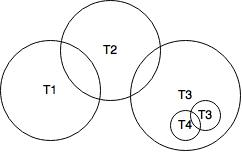
\includegraphics[]{VennDiagram.jpg}
\end{center}
\caption{A Typical Criterion}
\label{fig:venndiagram}
\end{figure}

A technique that Li.Zhang, Marinov, Lu.Zhang and Khurshid \cite{zhang2011empirical} examined was the use of a greedy technique in comparison to heuristics with the coverage information. A test requirement is set by the tester, for example using statement coverage. The idea for the greedy technique was that it would greedily select a test case that satisfies the maximum number of unsatisfied test requirements and would continue until all the test requirements had been satisfied. So the new test suite will contain exactly the same coverage as the old test suite while potentially removing redundant test cases. The heuristic implementation was first conceived by Harrold, Gupta and Soffa \cite{harrold1993methodology} where essential test cases are selected as early as possible. Essential being that only when one test case satisfies a test requirement exclusively. The heuristic approach resulted in the most cost-effective reduction showing that although greedy approach worked, there were better techniques available.

In situations it is not possible to generate a spectra to analyse, static analysing must be used to determine the level of redundancy. Robinson, Li and Francis \cite{li2008static} examine the possibility to do this. For the benchmark they use, the test cases are written in a high level automation framework and consists of a list of commands. The commands perform actions such as file copying and loading configurations. To identify redundant test cases, they examine the test cases commands as well as the instructions within the procedures it will load. To calculate the similarities between two test cases, they consider three different metrics, Manhattan distance, unigram cosine similarity and bigram cosine similarity. They each were measuring how closely related two tests were based on the sequence of commands and procedures loaded. There findings were similar to Maurer et al. \cite{koochakzadeh2009test} in that there are a large number of false - positives.

Static checking would provide useful information in such a framework where the dynamic data can not be collected. However, it would only work in a situation where the framework allows for the data to be examined in a static fashion such as the one used in \cite{li2008static}. Dynamic allows for more data to be collected and on more frameworks, allowing for more analysis to occur. The papers examined looked at the coverage of a test suite at several different criterion levels. But none looked at the method execution spectra. This leaves a potentially useful set of information that could be used to help determine the level of redundancy within a test suite. 